Farmer John has three farms lined up aloneside each other: $A, B, C$,
he invites all his cows from these farms to a dancing party on April Fools' Day.
During the party, Farmer John wants to count the attendance of cows from each farm,
but he can't directly ask their working farm because it's confidential.
Instead, Farmer John asks each cow to count the attendance of each farm, and he get the following results:
\begin{itemize}
  \item $A_1, B_1, C_1$
  \item $A_2, B_2, C_2$
  \item $\ldots$
  \item $A_n, B_n, C_n$
\end{itemize}
where $A_i, B_i, C_i$ is the attendance of each farm answered by the $i$th cow (include itself).

\begin{center}
  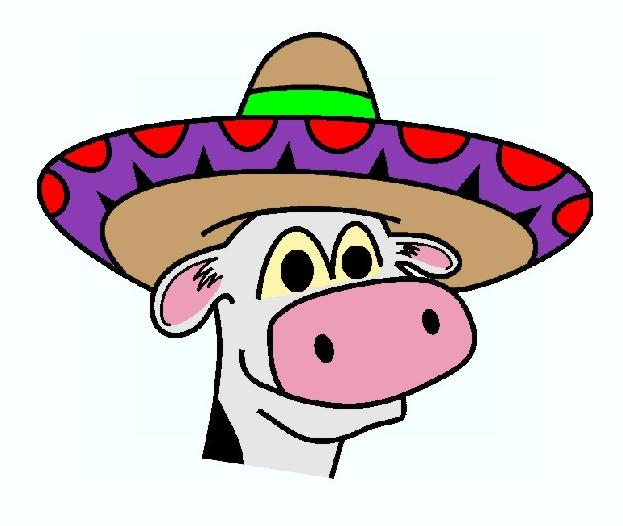
\includegraphics[scale=0.3, natwidth=623, natheight=526]{cows.jpg}
\end{center}

Farmer John knows the social habit of these cows very well, he assumes answers of cows satisfy following conditions:
\begin{itemize}
  \item cows never miscount the attendance for their \textbf{working farm}, because they know each other
  \item cows may underestimate (but never overestimate) the attendance for \textbf{adjacent farms}, because they don't know everyone very well
  \item cows from $A$ and $C$ can't count attendance of each other and the answer for that farm must be $0$, because they are too far away to know others 
  \item cows may decide to lie and give false answer, because it's April Fools' Day
\end{itemize}

Farmer John wonders that whether it is possible that all cows are telling truth or there must be some cows lying.
